%\section{Описание логической структуры}

\section{Выходной конфигурационный файл}

Так как результатом работы программы является сгенерированный конфигурационный файл, вначале рассмотрим его структуру и команды, используемые в нем.

Конфигурационный файл можно разделить на несколько блоков, отвечающих за настройку различных параметров:

\begin{itemize}
	\item блок начальной настройки;
	\item блок настройки интерфейсов;
	\item блок настройки VLAN;
	\item блок настройки маршрутизации;
	\item блок настройки DHCP;
	\item блок настройки NAT;
	\item блок настройки ACL.
\end{itemize}

В зависимости от типа устройства (маршрутизатор или коммутатор) в данном файле возможно наличие следующих блоков:

\begin{itemize}
	\item маршрутизатор:
	
	\begin{itemize}
		\item блок начальной настройки;
		\item блок настройки интерфейсов;
		\item блок настройки маршрутизации;
		\item блок настройки DHCP;
		\item блок настройки NAT;
		\item блок настройки ACL.
	\end{itemize}
	
	\item коммутатор:
	
	\begin{itemize}
		\item блок начальной настройки;
		\item блок настройки интерфейсов;
		\item блок настройки VLAN;
	\end{itemize}
\end{itemize}

\subsection{Начальная настройка}

Блок начальной настройки позволяет включает в себя команды\cite{cisco-command}:

\begin{itemize}
	\item указания имени оборудования
	
	\begin{lstlisting}
hostname <RouterN>
	\end{lstlisting}
	
	\item включения шифрования паролей
	
	\begin{lstlisting}
service password-encryption		
	\end{lstlisting}
	
	\item настройка приветственного сообщения
	
	\begin{lstlisting}
banner motd #Hello, this is graduate work of Cheretaev Ivan#
	\end{lstlisting}	
	
	\item установка пароля на консольное подключение
	
	\begin{lstlisting}
line console 0
exec-timeout 1440
password <password>
login
logging synchronous
	\end{lstlisting}
	
	\item установка пароля на терминальное подключение
	
\begin{lstlisting}
line console 0
exec-timeout 1440
password <password>
login
logging synchronous
transport input all
\end{lstlisting}
	
\end{itemize}


\subsection{Настройка интерфейсов}

Для настройки интерфейсов может использоваться следующий набор команд:
\begin{itemize}
	\item включение/выключение определенного интерфейса
	
\begin{lstlisting}
interface <type> <number>
<no> shutdown
\end{lstlisting}

	\item указание описания интерфейса
	
	\begin{lstlisting}
description <Description>
	\end{lstlisting}

	\item настройка порта для передачи нетегированного трафика, принадлежащего определенному VLAN'у
	
	\begin{lstlisting}
switchport mode access
switchport access vlan <vlanID>
	\end{lstlisting}
	
	\item настройка порта для передачи тегированного трафика одного или нескольких VLAN'ов 
	
	\begin{lstlisting}
switchport mode trunk
switchport trunk allowed vlan <vlanIDs>
	\end{lstlisting}
	
	\item IP-адрес 
	\begin{lstlisting}
ip address <IP-address> <IP-mask>
	\end{lstlisting}	
	
\end{itemize}

\subsection{VLAN}

Блок настройки VLAN обеспечивает создание требуемого количества VLAN, а также указание имени и описания VLAN.

\begin{lstlisting}
vlan <ID>
name <nameVLAN>
description <Description VLAN>
\end{lstlisting} 

\subsection{Маршрутизация}

Блок настройки маршрутизации позволяет настраивать статические маршруты, а также протоколы динамической маршрутизации OSPF и EIGRP.

\begin{itemize}
	\item статический маршрут
	\begin{lstlisting}
ip route <IP-network> <IP-mask> <interface or address next router>
	\end{lstlisting}
	
	\item OSPF
	
	\begin{itemize}
		\item включение OSPF
		
		\begin{lstlisting}
router ospf <Id>
		\end{lstlisting}
		
		\item прямое указание идентификатора маршрутизатора
		
\begin{lstlisting}
router-id <1.1.1.1>
\end{lstlisting}

\item добавление сети в объявления OSPF

\begin{lstlisting}
network <IP-network> <IP-wildcard_mask> area <areaID>
\end{lstlisting}
	\end{itemize}
		\item EIGRP
		
		\begin{itemize}
			\item включение EIGRP
			
			\begin{lstlisting}
router eigrp <Id>
			\end{lstlisting}
			
			\item прямое указание идентификатора маршрутизатора
			
			\begin{lstlisting}
router-id <1.1.1.1>
			\end{lstlisting}
			
			\item добавление сети в объявления EIGRP
			
			\begin{lstlisting}
network <IP-network> <IP-wildcard_mask> area <areaID>
			\end{lstlisting}
		\end{itemize}
\end{itemize}

\subsection{DHCP}

\begin{itemize}
	\item активация DHCP-сервера
	
	\begin{lstlisting}
service dhcp
	\end{lstlisting}
	
	\item настройка DHCP-пула на маршрутизаторе (аналогичным образом настраиваются пулы для каждой подсети) и указание шлюза по умолчанию для клиентов
	
	\begin{lstlisting}
ip dhcp pool guest                             
network <IP-address> <IP-mask>
default-router <IP-address>
	\end{lstlisting}
	
	\item исключение из пула IP-адреса
	
	\begin{lstlisting}
ip dhcp excluded-address <IP-address>
	\end{lstlisting}
\end{itemize}

\subsection{NAT}

\begin{itemize}
	\item определение интерфейса в качестве внутреннего интерфейса NAT.
	
	
\begin{lstlisting}
interface <type> <number>
ip nat inside
\end{lstlisting}

	\item определение интерфейса в качестве внешнего интерфейса NAT.
	
	
\begin{lstlisting}
interface <type> <number>
ip nat outside
\end{lstlisting}

\item  создание пула NAT 

\begin{lstlisting}
ip nat pool <poolName> <startIP-address> <endIP-address> prefix <prefix>
\end{lstlisting}

\item создание списка доступа

\begin{lstlisting}
access-list <id> permit <startIP-address> <endIP-address>
\end{lstlisting}

\item связывание списка доступа и пула NAT

\begin{lstlisting}
ip nat inside source list <id> pool <poolName>
\end{lstlisting}
\end{itemize}

\subsection{ACL}

Блок настройки ACL содержит команды, создающие списки контроля доступа и применяющие их к интерфейсам.

\begin{itemize}
	\item создание стандартного списка контроля доступа
	
\begin{lstlisting}
access-list <number from 1 to 99> {permit | deny | remark} {address | any | host} [source-wildcard]
\end{lstlisting}

\item создание расширенного списка контроля доступа

\begin{lstlisting}
access-list <number from 100 to 199> {permit | deny | remark} protocol source [source-wildcard] [operator operand] [port  <port> [established]
\end{lstlisting}
\end{itemize}

\section{Алгоритм работы программы}

Общий алгоритм программы можно представить в виде схемы, изображенной на рисунке \ref{fig:alghoritm}.

\begin{figure}[h!]
	\centering
	\includegraphics[width=0.9\linewidth]{pic/alghoritm}
	\caption{Схема работы программы}
	\label{fig:alghoritm}
\end{figure}

Далее осветим основные моменты, происходящие на данных этапах.

\subsection{Основное окно программы}

Основное окно программы представлено объектом класса \texttt{MainWindow}, наследуемом от \texttt{QMainWindow}\cite{qt:shlee}.

При запуске программы происходит чтение файла настроек программы, содержащего информацию об уже существующих шаблонах.

Для этого установим такой следующий синтаксис файла настроек:
\begin{lstlisting}[label=lst:structini,caption=Синтаксис файла настроек]
[template]
key=value
\end{lstlisting}
где \texttt{template} --- уникальное имя шаблона, \texttt{key} --- ключ, \texttt{value} --- значение ключа.

\lstinputlisting[label=lst:loadini,caption=Загрузка информации из ini-файла]{listing1.txt}

\subsection{Создание нового шаблона}

Окно создания нового шаблона представлено объектом класс \texttt{EditorWindow}, наследуемом от \texttt{QMainWindow}. На форме расположены элементы, обеспечивающие выбор пользователем необходимого функционала.

При сохранении шаблона происходит запись параметров шаблона в ini-файл (аналогично листингам \ref{lst:structini} и \ref{lst:loadini}).


\subsection{Редактирование шаблона}

Окно создания нового шаблона так же представлено объектом класс \texttt{EditorWindow}. 

При создании формы происходит установление значений элементов, в зависимости от значения записанного в ini-файл для данного шаблона (аналогично листингам \ref{lst:structini} и \ref{lst:loadini}).

При сохранении шаблона происходит запись параметров шаблона в ini-файл (аналогично листингам \ref{lst:structini} и \ref{lst:loadini}).

\subsection{Использование шаблона}

Окно использования шаблона представлено объектом класса \texttt{TemplateWindow}, наследуемом от \texttt{QMainWindow}.

Список элементов, присутствующих на форме, формируется в зависимости от параметров шаблона, записанных в ini-файле.

\subsection{Ввод необходимых параметров}

В программе организованы режимы проверки введенных данных.

Поскольку в режиме ввода команд в IOS допустимы только английские символы, в полях ввода ограничен ввод текста. Это сделано с использованием класса \texttt{WordValidator}, наследуемого от \texttt{QValidator}.Для реализации класса \texttt{QValidator} необходимо реализовать виртуальную функцию \texttt{validate(QString \&, int \&)}, что приведено в листинге \ref{lst:wordvalid}.

\begin{lstlisting}[label=lst:wordvalid,caption=Валидация введенного текста]
QValidator::State WordValidator::validate(QString &text, int &pos) const
{
	QRegExp regex("^([a-zA-Z0-9]+)*$");
	if (regex.exactMatch(text))
		return Acceptable;
	else return Invalid;
}
\end{lstlisting}

Аналогичным образом была реализована валидация вводимого текста в полях, где необходим был ввод текста (с пробелами). Для этого был создан класс \texttt{TextValidator}, так же наследуемый от \texttt{QValidator}.

Так как вышеописанный метод позволяет полностью ограничить ввод недопустимых символов, для валидации введенного IP-адреса и маски сети, он не подходит, поскольку иначе будет невозможно даже начать ввод IP-адреса. В этом случаем будем просто проверять текст при изменении, в случае, если он не будет валидным IP-адресом, обозначим данное поле ввода как некорректное (в соответствии с листингом \ref{lst:ipvalid} и рисунком \ref{fig:ipvalid}).

\begin{lstlisting}[label=lst:ipvalid,caption=Валидация IP-адреса]
Ipv4Validator *validator = new Ipv4Validator();
if (validator->validate(text, pos) == QValidator::Invalid)
	ui->ipv4edit->setStyleSheet("border: 1px solid red");
else ui->ipv4edit->setStyleSheet("");
\end{lstlisting}

\begin{figure}[th!]
\centering
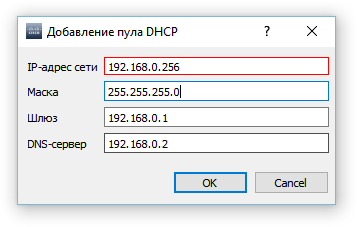
\includegraphics[width=0.8\linewidth]{pic/ipvalid}
\caption{Обозначение неправильного ввода}
\label{fig:ipvalid}
\end{figure}



\subsection{Генерация файла конфигурации}

Значения параметров маршрутизаторов, коммутаторов, интерфейсов, VLAN, DHCP, маршрутизации, NAT, ACL на протяжении работы программы хранятся в объектах класса \texttt{RouterModel}, \texttt{SwitchModel}, \texttt{InterfaceModel}, \texttt{VLANModel}, \texttt{DHCPModel}, \texttt{RouteModel}, \texttt{NATModel} и \texttt{ACLModel} соответственно, наследуемых от класса \texttt{ICiscoConfig}. Класс \texttt{ICiscoConfig} требует реализовать функцию \texttt{generetaeConfig}:

\begin{lstlisting}
virtual QString genereteConfig() = 0;
\end{lstlisting}

Вызов данной функции возвращает набор команд, необходимый для настройки соответствующего функционала.

Таким образом, после проверки правильности заполнения всех необходимых для ввода полей формы, производится запись в указанный пользователем файл значения функции \texttt{generateConfig()}.

%%\begin{lstlisting}
%%
%%!Writing Automated Startup
%%
%%enable
%%configure terminal
%%no ip domain-lookup
%%hostname hostname
%%enable secret class
%%end
%%\end{lstlisting}

%Исходя из схемы, представленной на рисунке \ref{fig:alghoritm}, выделяются 